% SCIENTIFIC COMPUTING
Modern engineering and scientific computing stimulate each other in a fruitful way.
This synergy has led to a number of great discoveries and breakthroughs,
e.g.\ the \emph{Monte Carlo method} \cite{MCMC:Metropolis1949} and the \emph{Kalman filter} \cite{Bayesian:Kalman1960,Bayesian:Kalman1961}.
Due to the steady increase and availability of computer capacities on the one hand and algorithmic advances on the other hand,
progress in computational science and engineering is nowadays made at an unprecedented pace.
Mature programming environments and ready-made software packages are available for a variety of dedicated tasks, e.g.\ for finite element analysis and multiphysics simulation.
The necessary processing power and computing time are provided by personal computers or high-performance computing clusters.
More and more complex systems can be simulated in an ever-increasing level of detail.
This trend continues to the present day.
\par % PARAMETER UNCERTAINTY
The accurate simulation of large-scale systems typically hinges on the knowledge of a great number of physical parameters.
In practice they are hardly known exactly, though.
Even if all parameters of a certain model could be specified somehow, this would not necessarily shield from systematic errors and guarantee satisfactory predictions.
Inadequacies are immanent in all physical models to some degree, e.g.\ due to missing physics or unresolved scales.
The investigation of different sources and levels of inaccuracy and imprecision in numerical simulations is therefore suggested.
This is the objective of \emph{uncertainty quantification} (UQ) \cite{Uncertainty:Smith2014,Uncertainty:Sullivan2015}.
\par % UNCERTAINTY QUANTIFICATION
In a wider sense, UQ deals with all uncertainties of computer simulations within an academic or industrial context.
One certainly encounters various quite different sources of error in scientific computing \cite{Uncertainty:Oberkampf2010,Uncertainty:MurraySmith2015}.
These include but are not limited to \emph{parameter uncertainty} \cite{Uncertainty:Rocquigny2008,Uncertainty:Rocquigny2012},
\emph{numerical inaccuracy} \cite{Computing:Higham2002,Computing:Deuflhard2003,Computing:Quarteroni2007}
and \emph{measurement noise} \cite{Uncertainty:Fornasini2008,Uncertainty:Gupta2012,Uncertainty:Grabe2014}.
While the two latter types of errors are treated in statistical and numerical analysis, UQ concentrates on the first-mentioned type in a narrower sense.
With this ambition, UQ has recently emerged as an active research field at the intersection of statistics, applied mathematics, computer science and engineering.
\par % PARAMETER UNCERTAINTY
In engineering applications, one commonly distinguishes between \emph{epistemic uncertainty} and \emph{aleatory variability} \cite{Uncertainty:Ayyub2006}.
The former refers to a lack of knowledge of the analyst, whereas the latter relates to a natural randomness of the system.
In statistical inference, \emph{frequentist} and \emph{Bayesian} interpretations of probability
differ in the way they address these uncertainties \cite{Statistics:Barnett1999,Statistics:Cox2006,Statistics:Samaniego2010}.
On the one hand, probabilities are only employed for describing objective frequencies.
On the other hand, they are also utilized for representing subjective ignorance.
While it is enjoyable to reflect and dispute about such a categorization, with good reason one may wonder whether it is really helpful or rather creates confusion.
Taking a pragmatic point of view and declining the related philosophical debates, the use of probability theory for either uncertainty is a common modeling choice in UQ.
\par % MODEL UNIVERSE
While the fundamentals of UQ are therefore well-established in principle, the actual challenge is the complexity of modern engineering problems.
The system under study is often composed of different interacting components, each of which may be already complex taken only by itself.
A complete model of this system usually consists of numerous deterministic and stochastic sub-models of the physics and uncertainty involved.
Abstractly one may speak of the ``model universe'' \cite{Uncertainty:Kiureghian2009} or ``theoretical world'' \cite{Statistics:Kass2011}
that embodies all assumptions and idealizations of that overall model.
In \cref{fig:UQ:ModelUniverse} it is attempted to illustrate this conception.
The goal of UQ then becomes the quantitative analysis and global management of uncertainty throughout the integrated system.
\par % FORWARD/INVERSE UQ
In a real-case scenario, the workflow typically involves a whole chain of intertwined UQ analyses.
Broadly speaking, these tasks can be divided into \emph{forward UQ}, i.e.\ characterizing the model outputs, and \emph{inverse UQ}, i.e.\ learning about the model inputs.
See \cref{fig:UQ:ForwardInverse} for a visualization.
In \emph{uncertainty propagation} \cite{Probability:Grigoriu2002,Probability:Grigoriu2012} one tries to find the full distribution of model outputs for given input uncertainties.
This includes \emph{reliability analysis} \cite{Uncertainty:Lemaire2009,Uncertainty:Nowak2013} where one focuses on the computation of the failure probability,
e.g.\ that the system output exceeds a certain threshold.
While these are forward UQ problems, \emph{parameter identification} \cite{Inversion:Tarantola2005,Inversion:Kaipio2005}
and \emph{data assimilation} \cite{Bayesian:Kalnay2002,Bayesian:Evensen2009} belong to inverse UQ.
Given noisy observations of the system output, the goal is the experimental estimation of unknown system parameters or dynamical states.
% FIGURES: MODEL UNIVERSE & FORWARD/INVERSE UQ
\begin{figure}[htbp]
  \begin{minipage}[c]{0.58\textwidth}
    \centering
    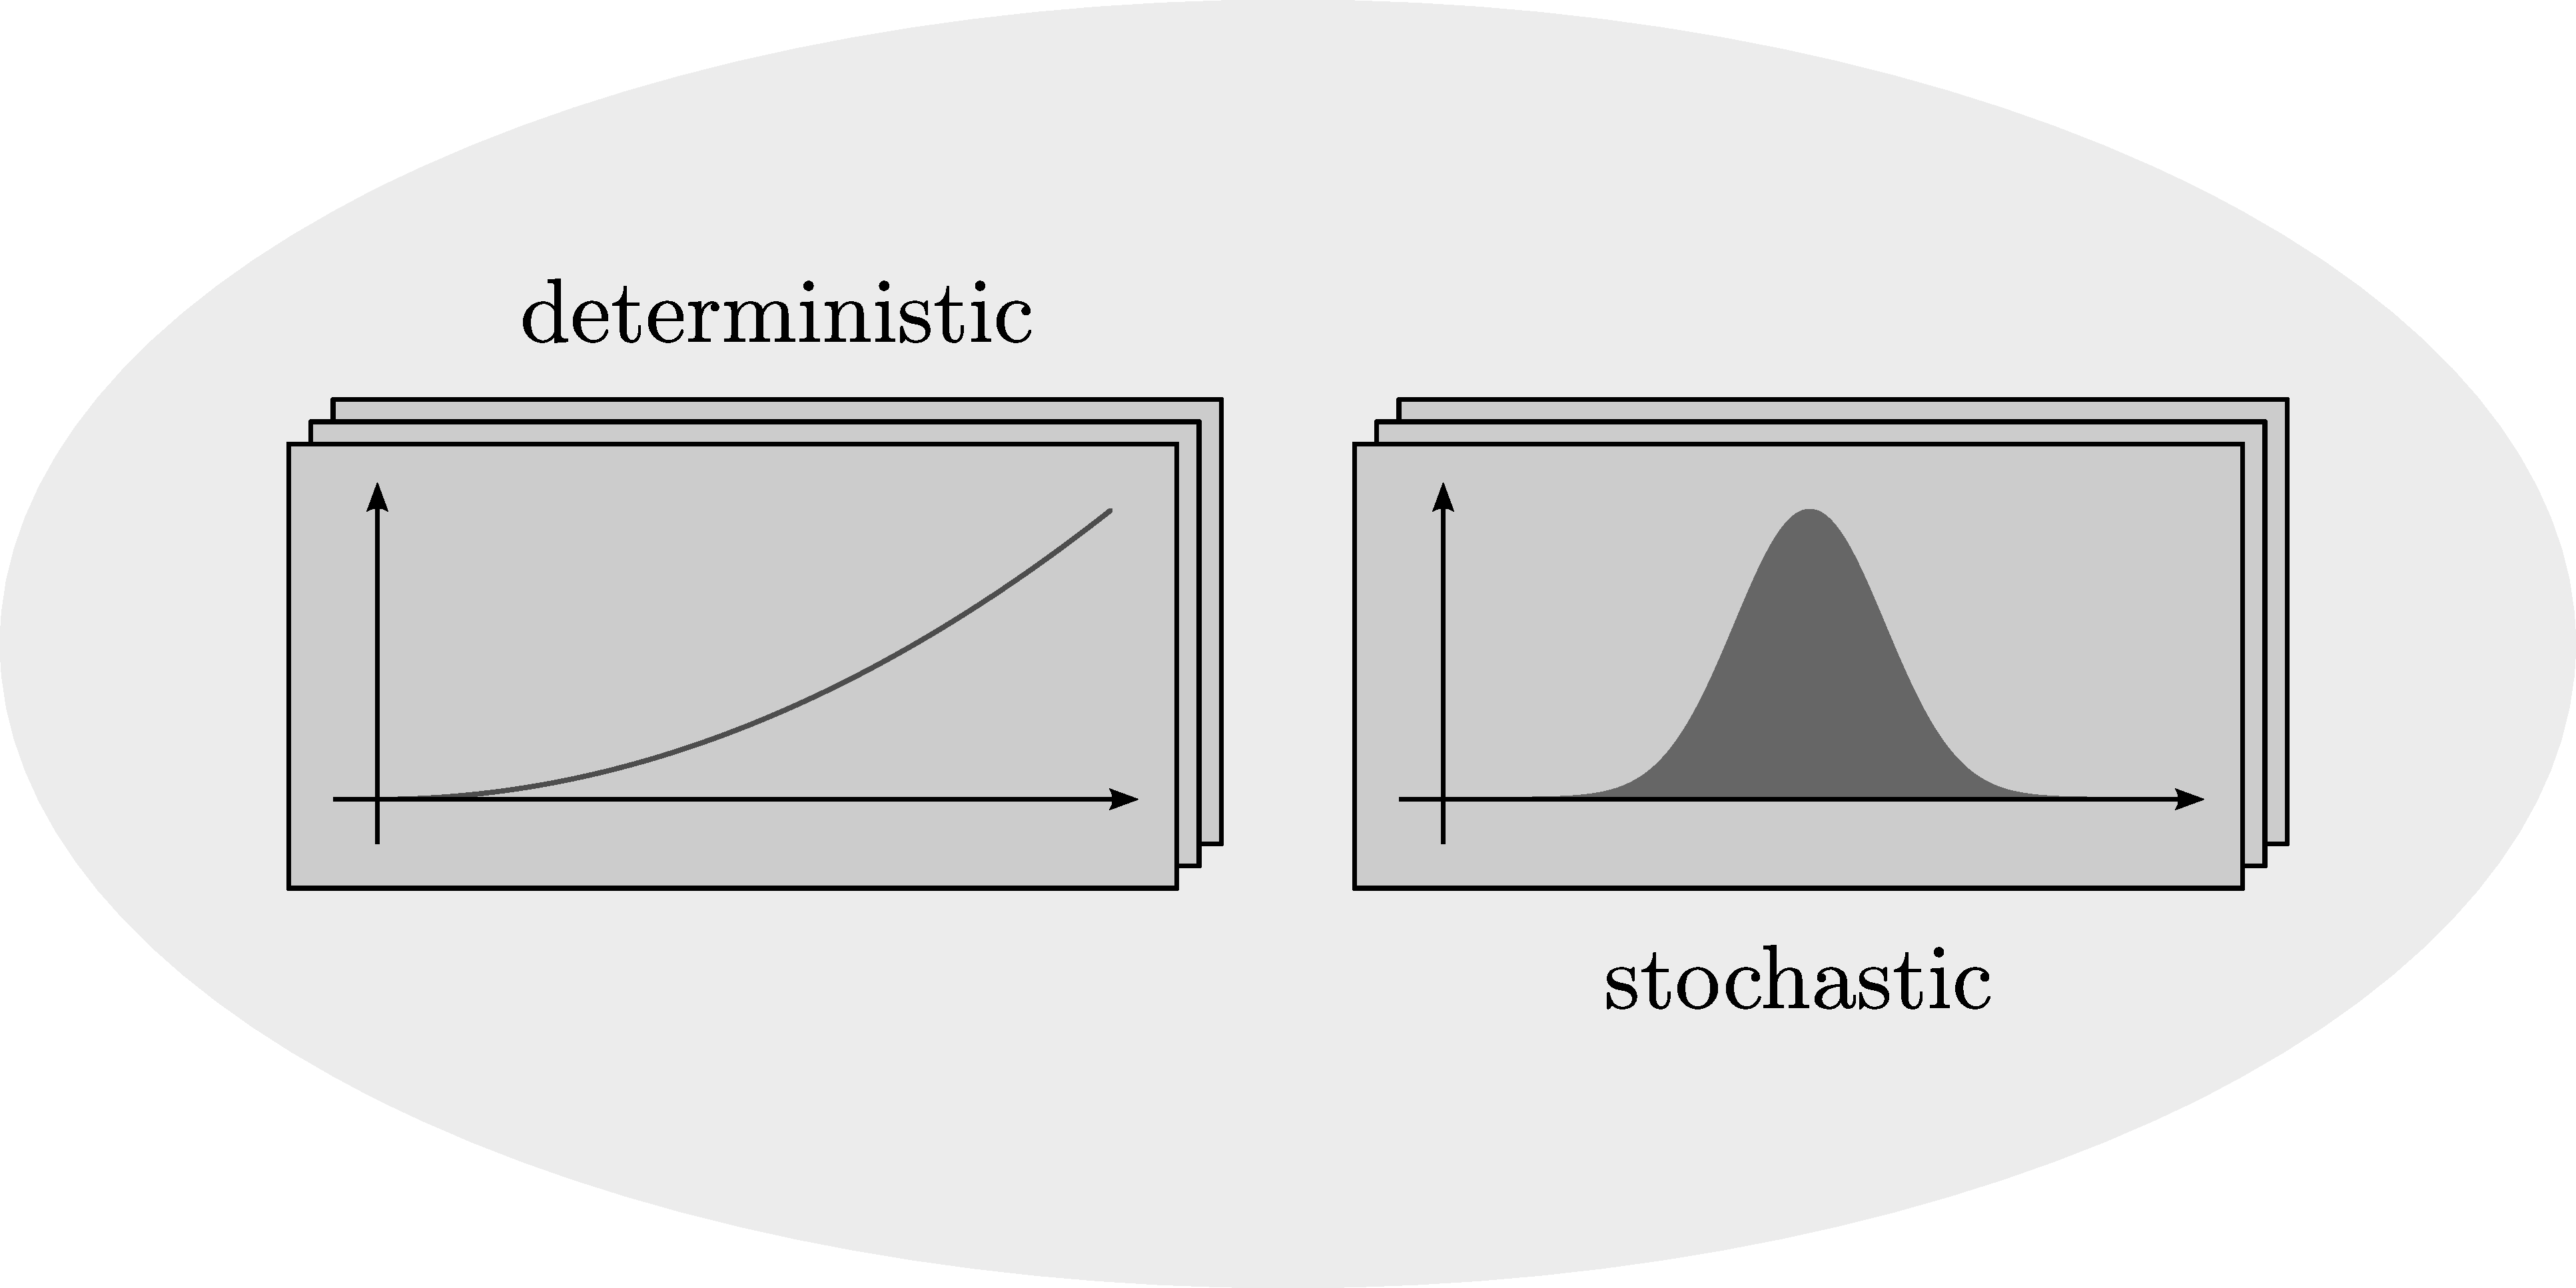
\includegraphics[width=\textwidth]{fig_UQ_ModelUniverse}
    \caption[Model universe]{Model universe.}
    \label{fig:UQ:ModelUniverse}
  \end{minipage}%
  \hfill%
  \begin{minipage}[c]{0.38\textwidth}
    \centering
    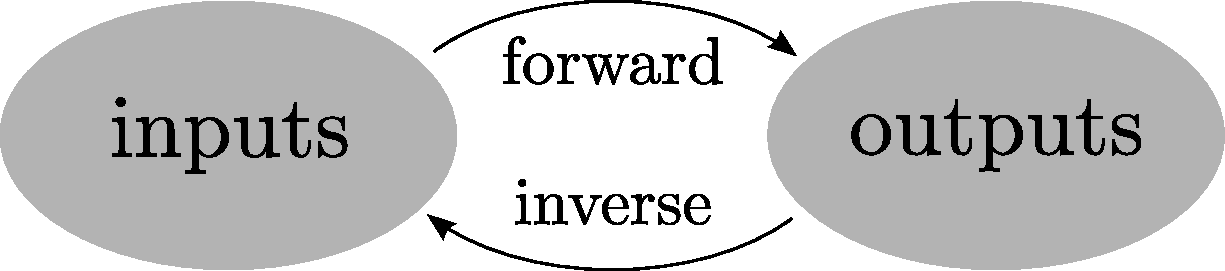
\includegraphics[width=\textwidth]{fig_UQ_ForwardInverse}
    \caption[Forward and inverse problems]{Forward and inverse problems.}
    \label{fig:UQ:ForwardInverse}
  \end{minipage}%
\end{figure}
\par % INTERMEDIATE UQ
There are also some intermediate UQ tasks that concentrate on understanding the input-output relationship that the model establishes.
By mimicking this relation or exploiting its structure one can accelerate forward as well as inverse UQ problems.
\emph{Surrogate modeling} \cite{Kriging:Fang2006,Kriging:Forrester2008} aims at an approximation of the model that is both easy to interpret and cheap to evaluate.
Similarly, \emph{model reduction} \cite{Uncertainty:Qu2004,Uncertainty:Antoulas2005}
subsumes techniques that try to simplify the model while a reasonable degree of accuracy is maintained.
In \emph{sensitivity analysis} \cite{Uncertainty:Saltelli2004,Uncertainty:Saltelli2008} one compares and ranks the importance of different inputs with respect to their effect on the outputs.
This allows one to identify the most and least influential parameters.
% FINAL OBJECTIVE
While many of the activities in between forward and inverse UQ are worthwhile by themselves, they still need to be seen in the bigger picture of
\emph{risk analysis} \cite{Uncertainty:Bedford2001,Uncertainty:Aven2012} and \emph{decision making} \cite{Uncertainty:Herrmann2015,Uncertainty:Kochenderfer2015}.
\par % OVERVIEW
The remainder of this introductory chapter is organized as follows.
Some fundamentals of uncertainty propagation are reviewed in \cref{sec:Uncertainty:UncertaintyPropagation}.
A discussion about local methods such as Taylor series approximations follows in \cref{sec:Uncertainty:TaylorApproximation}.
This eventually motivates global surrogate modeling approaches based on orthogonal polynomials in \cref{sec:Uncertainty:SurrogateModeling}.
Least squares minimization techniques for computing function approximations are subsequently presented in \cref{sec:Uncertainty:LeastSquares}.
Multivariate model outputs are considered in \cref{sec:Uncertainty:MultivariateOutput}.
Issues related to high-dimensionality and sparsity are finally discussed in \cref{sec:Uncertainty:CurseOfDimensionality}.